%% LyX 2.4.4 created this file.  For more info, see https://www.lyx.org/.
%% Do not edit unless you really know what you are doing.
\documentclass[english,t]{beamer}
\usepackage{mathptmx}
\usepackage[T1]{fontenc}
\usepackage[latin9]{inputenc}
\usepackage{amssymb}
\usepackage{cancel}

\makeatletter

%%%%%%%%%%%%%%%%%%%%%%%%%%%%%% LyX specific LaTeX commands.
%% Because html converters don't know tabularnewline
\providecommand{\tabularnewline}{\\}

%%%%%%%%%%%%%%%%%%%%%%%%%%%%%% Textclass specific LaTeX commands.
% this default might be overridden by plain title style
\newcommand\makebeamertitle{\frame{\maketitle}}%
% (ERT) argument for the TOC
\AtBeginDocument{%
  \let\origtableofcontents=\tableofcontents
  \def\tableofcontents{\@ifnextchar[{\origtableofcontents}{\gobbletableofcontents}}
  \def\gobbletableofcontents#1{\origtableofcontents}
}

%%%%%%%%%%%%%%%%%%%%%%%%%%%%%% User specified LaTeX commands.
\usetheme{Warsaw}
% or ...

\setbeamercovered{transparent}
% or whatever (possibly just delete it)
\setbeamercovered{invisible} %makes overlays invisible

%gets rid of navigation symbols
\setbeamertemplate{navigation symbols}{}

%\usepackage{hyperref}
%\usepackage[usenames,dvipsnames,table]{xcolor} %adds additional color options
\definecolor{links}{HTML}{2A1B81}
%\hypersetup{colorlinks,linkcolor=blue,urlcolor=links}

\usepackage{multicol}

\usepackage{tikz}
\usetikzlibrary{calc}
\usetikzlibrary{plotmarks}
\usetikzlibrary{shapes}
\usepackage{pgfplots}
\pgfplotsset{compat=newest}

\usepackage{forest} %%for tree diagram

\usepackage{calc}
\usepackage[nomessages]{fp}

\usepackage[super]{nth} %easy 1st, 2nd, etc

%\usepackage{advdate}    % Advancing/saving dates
\usepackage{datetime}   % Dates formatting
%\usepackage{datenumber} % Counters for dates

\usepackage[super]{nth}

\usepackage{etex}

\usepackage{fancybox}

%%table colors
%\usepackage[table]{xcolor}
\usepackage{colortbl}

\usepackage[outline]{contour}  %allows text halos

\usepackage{epsdice} %%dice font
\usepackage[misc]{ifsym}
\newfont\dice{dice3d} %%3d dice font

\contourlength{1pt} %sets halo width
%%example: \node at (0.75,0.5) {\contour{white}{\Large Text!}};
%%example:  \node [fill=white,inner sep=1pt] at (2.25,0.5) {\Large 			Text!};
%%example:  \node [fill=white,rounded corners=2pt,inner sep=1pt] at 			(3.75,0.5) {\Large Text!};

%%%%%%%%%%%%%%%%%%%%%%%%%%%
\def\formatdateny{\csname noyear\languagename\expandafter\endcsname\formatdate}
\def\noyearenglish#1, \the\@year{#1}
\let\noyearamerican\noyearenglish
\let\noyearbritish\noyearenglish

%%allows uncover with forest diagrams
\tikzset{
    invisible/.style={opacity=0,text opacity=0},
    visible on/.style={alt=#1{}{invisible}},
    alt/.code args={<#1>#2#3}{%
      \alt<#1>{\pgfkeysalso{#2}}{\pgfkeysalso{#3}} % \pgfkeysalso doesn't change the path
    },
}
\forestset{
  visible on/.style={
    for tree={
      /tikz/visible on={#1},
      edge={/tikz/visible on={#1}}}}}

%%%redefines column alignment to match vertically
%\define@key{beamerframe}{t}[true]{% top
  %\beamer@frametopskip=.2cm plus .5\paperheight\relax%
  %\beamer@framebottomskip=0pt plus 1fill\relax%
 % \beamer@frametopskipautobreak=\beamer@frametopskip\relax%
  %\beamer@framebottomskipautobreak=\beamer@framebottomskip\relax%
  %\def\beamer@initfirstlineunskip{}%
%}

%%provides pdf with 4 slides per page; don't forget to add 'handout' to remove overlays
%\usepackage{pgfpages}
%\pgfpagesuselayout{4 on 1}[a4paper, landscape, border shrink=7mm]
%\pgfpageslogicalpageoptions{1}{border code=\pgfusepath{stroke}}
%\pgfpageslogicalpageoptions{2}{border code=\pgfusepath{stroke}}
%\pgfpageslogicalpageoptions{3}{border code=\pgfusepath{stroke}}
%\pgfpageslogicalpageoptions{4}{border code=\pgfusepath{stroke}}
%%%Don't forget to add 'handout'

\makeatother

\usepackage{babel}
\begin{document}
\newcommand{\xmax}{2000}
\newcommand{\xmin}{0}
\newcommand{\xstep}{0} %must be xmin+n
\newcommand{\ymax}{500}
\newcommand{\ymin}{0}
\newcommand{\ystep}{0} %must be ymin+n

\newcounter{countEx} \setcounter{countEx}{0}
\newcounter{countProb} \setcounter{countProb}{0}
\resetcounteronoverlays{countEx} \resetcounteronoverlays{countProb}

\newcommand{\ex}[3]{
	\addtocounter{countEx}{1}
	\only<#1-#2>{\begin{exampleblock} {Example \chNum.\secNum.\arabic{countEx}.} #3	\end{exampleblock}}
}

\newcommand{\prob}[4]{
	\addtocounter{countProb}{1}
	\only<#1-#2>{\begin{exampleblock} {Problem  \chNum.\secNum.\arabic{countProb}.\,#3} #4	\end{exampleblock}}
}

\newcommand{\yline}[4]{
	(#2 - #4)/(#1 - #3)*(x - #1) + #2
}

\beamerdefaultoverlayspecification{<+->}

%%%%Chapter and Section numbers%%%%%
\newcommand{\chNum}{3}
\newcommand{\secNum}{3 part 2}
\newcommand{\secTitle}{"And"}
\date{\formatdate{13}{10}{2014}}

\title[Section \chNum.\secNum: \secTitle]{Section \chNum.\secNum: \secTitle}

\subtitle{Finite Mathematics~~MTH 107~~Fall 2014}

\author{Dr.\,James Ashe}

\titlegraphic{\includegraphics[height=2.75cm]{/home/jim/JamesAshe/MHU/images/MarsHilUniversityLogo-Virtical.png}}

\institute{Mars Hill University}

\makebeamertitle 

%%True false command
\newcommand{\T}{\textcolor{green}{\contour{black}{T}}}
\newcommand{\F}{\textcolor{red}{\contour{black}{F}}}
\newcommand{\uT}[2]{\uncover<#1-#2>{\T}}
\newcommand{\uF}[2]{\uncover<#1-#2>{\F}}

%tkiz ball item 
\newcommand*\circled[1]{\tikz[baseline=(char.base)]
	{\node[circle,ball color=green!50!black!100, shade,   color=white,inner sep=1.2pt] (char) {\tiny #1};
	}
}
\subtitle{Venn Diagrams and the Product Rule\\
Section 3.3 and 3.6}
\makebeamertitle
\begin{frame}{Review/Preview: 3 ``and'' Problems}

\ex{1}{}{John has green, red, and blue pants; and a green and red shirt. What is the probability that he randomly selects blue pants \textbf{and} a blue shirt?}

\vspace{-.25cm}
\begin{columns}


\column{5.5cm}

\forestset{  
	L1/.style={rectangle, rounded corners, shade, top color=white,     bottom color=blue!50!black!20, draw=blue!40!black!60, very     thick},   	
	L2/.style={rectangle, rounded corners, shade, top color=white,     bottom color=blue!50!black!20, draw=blue!40!black!60, very     thick,
		edge={black,line width=1.15pt,line cap=round}},   	
	L3/.style={rectangle, rounded corners, shade, top color=white,     bottom color=blue!50!black!20, draw=blue!40!black!60, very     thick,
		edge={black,line width=1.15pt,line cap=round}},   	
	L4/.style={rectangle, rounded corners, shade, top color=white,     bottom color=blue!50!black!20, draw=blue!40!black!60, very     thick,
	edge={black,line width=1.15pt,line cap=round}}, 
}

\begin{forest}     
	for tree={
		scale=.75,        
		grow=0,
		reversed, %tree direction         
		parent anchor=east,
		child anchor=west, %edge anchors   		edge={line cap=round},
		outer sep=+1pt, %edge/node connection  		rounded corners,
		minimum width=15mm,
		minimum height=8mm, %node shape         l 		sep=10mm %level distance     
		}   
[Start,L1,for children={visible on=<2->}
	[Green Pants,L2, for children={visible on=<3->}         
		[Green Shirt,L3,for children={visible on=<3->}                     
		]         
		[Blue Shirt,L3,for children={visible on=<3->}            
		]               
	]     
	[Red Pants,L2,for children={visible on=<3->}         
		[Green Shirt,L3,for children={visible on=<3->}                     
		]         
		[Blue Shirt,L3,for children={visible on=<3->}           
		]               
	] 
	[Blue Pants,L2,for children={visible on=<3->}         
		[Green Shirt,L3,for children={visible on=<6->}            
		]         
		[Blue Shirt,L3,for children={visible on=<3->}           
		]               
	] 
] 
\end{forest}

\column{5.5cm}
\begin{itemize}
\item []<1->$P(BP\cap BS)$
\item []<2-> \hspace{12pt}$=\frac{1}{3}$\only<3->{$\times$ $\frac{1}{2}$} \only<4->{$=\frac{1}{6}$}
\item <5->The \nth{1} event does not affect the probability of the \nth{2}
event.
\item <6->These events are called \emph{independent}.
\end{itemize}
\end{columns}
\end{frame}

\begin{frame}{Review/Preview: 3 ``and'' Problems}

\textbf{Find the probability of the following:}\vspace{-.5cm}
\begin{columns}


\column{3.75cm}

\ex{5}{}{A king \textbf{and} a heart is drawn.}

\uncover<6->{$\frac{4}{52}$} \only<7->{$\times\frac{13}{52}$} \only<8->{$=\frac{1}{52}$}

\column{3.75cm}

\ex{5}{}{A king \textbf{and} \textbf{then} a heart is drawn with
replacement.}

\uncover<9->{$\frac{4}{52}$} \only<9->{$\times\frac{13}{52}$} \only<10->{$=\frac{52}{2704}=\frac{1}{52}$}

\column{3.75cm}

\ex{5}{}{A king \textbf{and then} a heart is drawn without replacement.}

\uncover<11->{drawing a non-heart king and heart 

\textbf{OR }

drawing a king of hearts and a heart.}

\uncover<12->{$\left(\frac{3}{52}\times\frac{13}{51}\right)+\left(\frac{1}{52}\times\frac{12}{51}\right)$}

\uncover<13->{$=\frac{51}{2652}\approx0.019$}
\end{columns}
\vspace{-.25cm}

\begin{columns}


\column{3.75cm}

\vspace{-70pt}
\begin{block}<2->{Conditional Probability.}
\small

\[
p(A\mid B)=\frac{n(A\cap B)}{n(B)}
\]

Probability of $A$ if \textbf{$B$ }has occurred.
\end{block}

\column{3.75cm}

\vspace{-70pt}
\begin{block}<4->{Product Rule}
\small$p(A\cap B)=p(A\mid B)\cdot p(B)$
\end{block}

\column{3.75cm}

\end{columns}
\end{frame}

\begin{frame}{Review/Preview: 3 ``and'' Problems}

\textbf{Find the probability of the following:}\vspace{-.5cm}
\begin{columns}


\column{3.75cm}

\ex{2}{}{A king \textbf{and} heart is drawn.}

\column{3.75cm}

\ex{2}{}{A king \textbf{and then} a heart is drawn with replacement.}

\column{3.75cm}

\ex{2}{}{A king \textbf{and then} a heart is drawn without replacement.}
\end{columns}
\vspace{-.25cm}
\begin{columns}


\column{3.75cm}

\vphantom{HI}\uncover<3->{$P(K\cap H)$}  \uncover<7->{$=\frac{1}{52}$}

 \only<4-4>{%%%% M or A %%%%%
\begin{center}
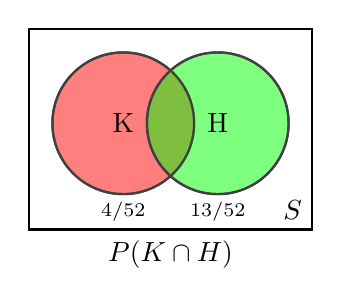
\begin{tikzpicture}[scale=.6]
	\def\circleA{(0,0) circle (1.5)} %A
	\def\circleB{(0:2) circle (1.5)} %B

	\colorlet{circle edgeA}{black!75} 
	\colorlet{circle areaA}{red!100}
	\colorlet{circle edgeB}{black!75} 
	\colorlet{circle areaB}{green!100}

	\tikzset{
		filledA/.style={fill=circle areaA, draw=circle edgeA, thick},
		filledB/.style={fill=circle areaB, draw=circle edgeB, thick},
		outlineA/.style={draw=circle edgeA, thick},
		outlineB/.style={draw=circle edgeB, thick},
	}
	
	\begin{scope}[fill opacity=0.5]         
			\fill[filledA] \circleA;
			\fill[filledB] \circleB;    
	\end{scope}

	\draw[outlineA] \circleA node[] {K} node[below=-1pt] at (0,-1.5) {\scriptsize $4/52$}; 
	\draw[outlineB] \circleB node[] {H} node[below=-1pt] at (2,-1.5) {\scriptsize $13/52$};
	%\draw (1,0) node {.25};
	\draw[thick] (-2,-2.25) rectangle (4,2) node[anchor=south east] at (current bounding box.south east) {$S$}; 
	\node[anchor=north] at (current bounding box.south) {$P(K\cap H)$}; 
\end{tikzpicture}
\end{center}} \only<5-5>{%%%% M or A with int label%%%%%
\begin{center}
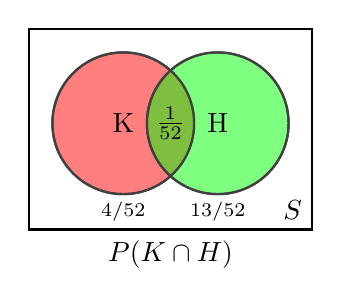
\begin{tikzpicture}[scale=.6]
	\def\circleA{(0,0) circle (1.5)} %A
	\def\circleB{(0:2) circle (1.5)} %B

	\colorlet{circle edgeA}{black!75} 
	\colorlet{circle areaA}{red!100}
	\colorlet{circle edgeB}{black!75} 
	\colorlet{circle areaB}{green!100}

	\tikzset{
		filledA/.style={fill=circle areaA, draw=circle edgeA, thick},
		filledB/.style={fill=circle areaB, draw=circle edgeB, thick},
		outlineA/.style={draw=circle edgeA, thick},
		outlineB/.style={draw=circle edgeB, thick},
	}
	
	\begin{scope}[fill opacity=0.5]         
			\fill[filledA] \circleA;
			\fill[filledB] \circleB;    
	\end{scope}

	\draw[outlineA] \circleA node[] {K} node[below=-1pt] at (0,-1.5) {\scriptsize $4/52$}; 
	\draw[outlineB] \circleB node[] {H} node[below=-1pt] at (2,-1.5) {\scriptsize $13/52$};
	\draw (1,0) node {$\frac{1}{52}$};
	\draw[thick] (-2,-2.25) rectangle (4,2) node[anchor=south east] at (current bounding box.south east) {$S$}; 
	\node[anchor=north] at (current bounding box.south) {$P(K\cap H)$}; 
\end{tikzpicture}
\end{center}} \only<6->{%%%% MnA with int label%%%%%
\begin{center}
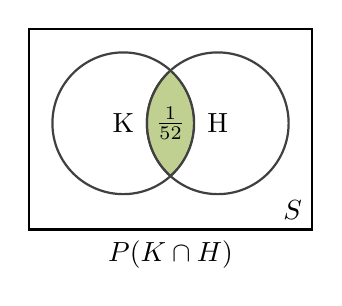
\begin{tikzpicture}[scale=.6]
	\def\circleA{(0,0) circle (1.5)} %A
	\def\circleB{(0:2) circle (1.5)} %B

	\colorlet{circle edgeA}{black!75} 
	\colorlet{circle areaA}{red!37}
	\colorlet{circle edgeB}{black!75} 
	\colorlet{circle areaB}{green!100}

	\tikzset{
		filledA/.style={fill=circle areaA, draw=circle edgeA, thick},
		filledB/.style={fill=circle areaB, draw=circle edgeB, thick},
		outlineA/.style={draw=circle edgeA, thick},
		outlineB/.style={draw=circle edgeB, thick},
	}
	
	\begin{scope}[fill opacity=0.5]    
		\clip \circleA;     
			\fill[filledB] \circleB;
		\clip \circleB;     
			\fill[filledA] \circleA;
	\end{scope}

	\draw[outlineA] \circleA node[] {K} node[below=-1pt] at (0,-1.5) {\scriptsize }; 
	\draw[outlineB] \circleB node[] {H} node[below=-1pt] at (2,-1.5) {\scriptsize };
	\draw (1,0) node {$\frac{1}{52}$};
	\draw[thick] (-2,-2.25) rectangle (4,2) node[anchor=south east] at (current bounding box.south east) {$S$}; 
	\node[anchor=north] at (current bounding box.south) {$P(K\cap H)$}; 
\end{tikzpicture}
\end{center}}

\column{3.75cm}

\vphantom{HI}\uncover<7->{$P(K\cap H)$}\uncover<11->{$=\frac{1}{52}$}

 \only<8-8>{%%%% M or A %%%%%
\begin{center}
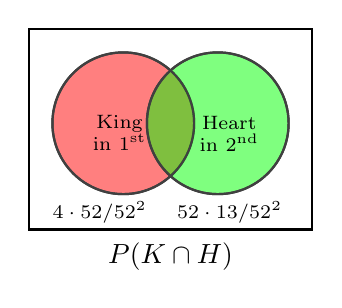
\begin{tikzpicture}[scale=.6]
	\def\circleA{(0,0) circle (1.5)} %A
	\def\circleB{(0:2) circle (1.5)} %B

	\colorlet{circle edgeA}{black!75} 
	\colorlet{circle areaA}{red!100}
	\colorlet{circle edgeB}{black!75} 
	\colorlet{circle areaB}{green!100}

	\tikzset{
		filledA/.style={fill=circle areaA, draw=circle edgeA, thick},
		filledB/.style={fill=circle areaB, draw=circle edgeB, thick},
		outlineA/.style={draw=circle edgeA, thick},
		outlineB/.style={draw=circle edgeB, thick},
	}
	
	\begin{scope}[fill opacity=0.5]         
			\fill[filledA] \circleA;
			\fill[filledB] \circleB;    
	\end{scope}

	\draw[outlineA] \circleA node[] {\scriptsize King \hspace{5pt}} node[below] {\scriptsize in \nth{1} \hspace{5pt}} node[below=-1pt] at (-.5,-1.5) {\scriptsize $4\cdot 52/52^2$};; 
	\draw[outlineB] \circleB node[] {\hspace{5pt} \scriptsize Heart} node[below] {\hspace{5pt} \scriptsize in \nth{2}} node[below=-1pt] at (2.25,-1.5) {\scriptsize $52\cdot 13/52^2$};
	%\draw (1,0) node {.25};
	\draw[thick] (-2,-2.25) rectangle (4,2) node[anchor=south east] at (current bounding box.south east) {$$}; 
	\node[anchor=north] at (current bounding box.south) {$P(K\cap H)$}; 
\end{tikzpicture}
\end{center}} \only<9-9>{%%%% M or A %%%%%
\begin{center}
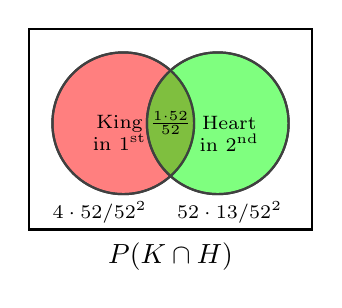
\begin{tikzpicture}[scale=.6]
	\def\circleA{(0,0) circle (1.5)} %A
	\def\circleB{(0:2) circle (1.5)} %B

	\colorlet{circle edgeA}{black!75} 
	\colorlet{circle areaA}{red!100}
	\colorlet{circle edgeB}{black!75} 
	\colorlet{circle areaB}{green!100}

	\tikzset{
		filledA/.style={fill=circle areaA, draw=circle edgeA, thick},
		filledB/.style={fill=circle areaB, draw=circle edgeB, thick},
		outlineA/.style={draw=circle edgeA, thick},
		outlineB/.style={draw=circle edgeB, thick},
	}
	
	\begin{scope}[fill opacity=0.5]         
			\fill[filledA] \circleA;
			\fill[filledB] \circleB;    
	\end{scope}

	\draw[outlineA] \circleA node[] {\scriptsize King \hspace{5pt}} node[below] {\scriptsize in \nth{1} \hspace{5pt}} node[below=-1pt] at (-.5,-1.5) {\scriptsize $4\cdot 52/52^2$};; 
	\draw[outlineB] \circleB node[] {\hspace{5pt} \scriptsize Heart} node[below] {\hspace{5pt} \scriptsize in \nth{2}} node[below=-1pt] at (2.25,-1.5) {\scriptsize $52\cdot 13/52^2$};
	\draw (1,0) node {\scriptsize $\frac{1\cdot 52}{52}$};
	\draw[thick] (-2,-2.25) rectangle (4,2) node[anchor=south east] at (current bounding box.south east) {$$}; 
	\node[anchor=north] at (current bounding box.south) {$P(K\cap H)$}; 
\end{tikzpicture}
\end{center}} \only<10->{%%%% MnA with int label%%%%%
\begin{center}
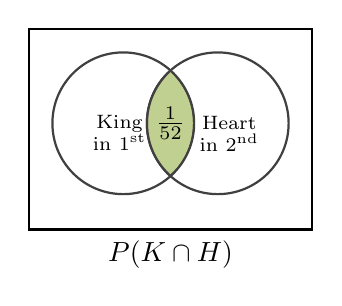
\begin{tikzpicture}[scale=.6]
	\def\circleA{(0,0) circle (1.5)} %A
	\def\circleB{(0:2) circle (1.5)} %B

	\colorlet{circle edgeA}{black!75} 
	\colorlet{circle areaA}{red!37}
	\colorlet{circle edgeB}{black!75} 
	\colorlet{circle areaB}{green!100}

	\tikzset{
		filledA/.style={fill=circle areaA, draw=circle edgeA, thick},
		filledB/.style={fill=circle areaB, draw=circle edgeB, thick},
		outlineA/.style={draw=circle edgeA, thick},
		outlineB/.style={draw=circle edgeB, thick},
	}
	
	\begin{scope}[fill opacity=0.5]    
		\clip \circleA;     
			\fill[filledB] \circleB;
		\clip \circleB;     
			\fill[filledA] \circleA;
	\end{scope}

	\draw[outlineA] \circleA node[] {\scriptsize King \hspace{5pt}} node[below] {\scriptsize in \nth{1} \hspace{5pt}} node[below=-1pt] at (-.5,-1.5) {\scriptsize $$};; 
	\draw[outlineB] \circleB node[] {\hspace{5pt} \scriptsize Heart} node[below] {\hspace{5pt} \scriptsize in \nth{2}} node[below=-1pt] at (2.25,-1.5) {\scriptsize $$};
	\draw (1,0) node {$\frac{1}{52}$};
	\draw[thick] (-2,-2.25) rectangle (4,2) node[anchor=south east] at (current bounding box.south east) {$$}; 
	\node[anchor=north] at (current bounding box.south) {$P(K\cap H)$}; 
\end{tikzpicture}
\end{center}}

\column{3.75cm}

\vphantom{HI}\uncover<12->{$P(K\cap H)$}\uncover<12->{$=\frac{51}{2652}$}

\only<13-13>{%%%% M or A %%%%%
\begin{center}
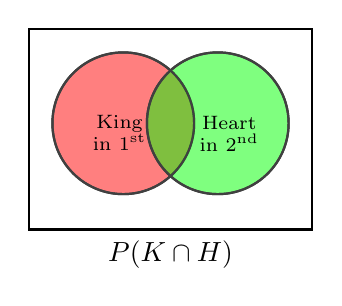
\begin{tikzpicture}[scale=.6]
	\def\circleA{(0,0) circle (1.5)} %A
	\def\circleB{(0:2) circle (1.5)} %B

	\colorlet{circle edgeA}{black!75} 
	\colorlet{circle areaA}{red!100}
	\colorlet{circle edgeB}{black!75} 
	\colorlet{circle areaB}{green!100}

	\tikzset{
		filledA/.style={fill=circle areaA, draw=circle edgeA, thick},
		filledB/.style={fill=circle areaB, draw=circle edgeB, thick},
		outlineA/.style={draw=circle edgeA, thick},
		outlineB/.style={draw=circle edgeB, thick},
	}
	
	\begin{scope}[fill opacity=0.5]         
			\fill[filledA] \circleA;
			\fill[filledB] \circleB;    
	\end{scope}

	\draw[outlineA] \circleA node[] {\scriptsize King \hspace{5pt}} node[below] {\scriptsize in \nth{1} \hspace{5pt}} node[below=-1pt] at (-.5,-1.5) {\scriptsize $$};; 
	\draw[outlineB] \circleB node[] {\hspace{5pt} \scriptsize Heart} node[below] {\hspace{5pt} \scriptsize in \nth{2}} node[below=-1pt] at (2.25,-1.5) {\scriptsize $$};
	%\draw (1,0) node {\scriptsize $\frac{1\cdot 52}{52}$};
	\draw[thick] (-2,-2.25) rectangle (4,2) node[anchor=south east] at (current bounding box.south east) {$$}; 
	\node[anchor=north] at (current bounding box.south) {$P(K\cap H)$}; 
\end{tikzpicture}
\end{center}} \only<14-14>{%%%% M or A %%%%%
\begin{center}
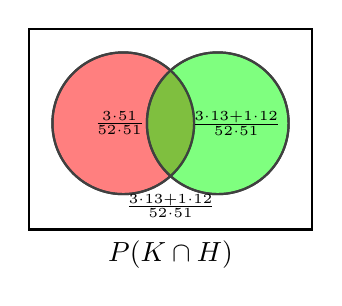
\begin{tikzpicture}[scale=.6]
	\def\circleA{(0,0) circle (1.5)} %A
	\def\circleB{(0:2) circle (1.5)} %B

	\colorlet{circle edgeA}{black!75} 
	\colorlet{circle areaA}{red!100}
	\colorlet{circle edgeB}{black!75} 
	\colorlet{circle areaB}{green!100}

	\tikzset{
		filledA/.style={fill=circle areaA, draw=circle edgeA, thick},
		filledB/.style={fill=circle areaB, draw=circle edgeB, thick},
		outlineA/.style={draw=circle edgeA, thick},
		outlineB/.style={draw=circle edgeB, thick},
	}
	
	\begin{scope}[fill opacity=0.5]         
			\fill[filledA] \circleA;
			\fill[filledB] \circleB;    
	\end{scope}

	\draw[outlineA] \circleA node[] {\scriptsize $\frac{3\cdot 51}{52\cdot 51}$ \hspace{5pt}} node[below=-1pt] at (-.5,-1.5) {};; 
	\draw[outlineB] \circleB node[] {\hspace{10pt} \scriptsize $\frac{3\cdot 13+1\cdot 12}{52\cdot 51}$} node[below=-1pt] at (2.25,-1.5) {\scriptsize $$};
	\draw (1,-1.75) node {\tiny $\frac{3\cdot 13 + 1\cdot 12}{52\cdot 51}$};
	\draw[thick] (-2,-2.25) rectangle (4,2) node[anchor=south east] at (current bounding box.south east) {$$}; 
	\node[anchor=north] at (current bounding box.south) {$P(K\cap H)$}; 
\end{tikzpicture}
\end{center}}
\end{columns}
\end{frame}

\begin{frame}{Probabilities and Venn Diagrams}

\vspace{-.5cm}
\begin{columns}


\column{5.5cm}

\ex{1}{}{The probability that a student \emph{passes} Art is 75\%,
\emph{fails} Math is 65\%, and \emph{passes} at least one is 85\%.
Find that a student:
\begin{itemize}
\item [a.]passes Math.
\item <5->[b.]passes both.
\item <11->[c.]fails both.
\item <15->[d.]passes only one. 
\end{itemize}
}

\column{5.5cm}

\vspace{.5cm}\only<2-2>{%%%%M'%%%%%
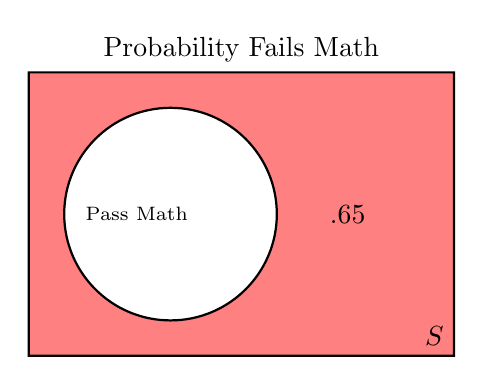
\begin{tikzpicture}[scale=.9]
	\def\circleA{(0,0) circle (1.5)} %A
	\def\circleB{(0:2) circle (1.5)} %B

	\colorlet{circle edgeA}{black!75} 
	\colorlet{circle areaA}{red!100}
	\colorlet{circle edgeB}{black!75} 
	\colorlet{circle areaB}{blue!100}

	\tikzset{
		filledA/.style={fill=circle areaA, draw=circle edgeA, thick},
		filledB/.style={fill=circle areaB, draw=circle edgeB, thick},
		outlineA/.style={draw=circle edgeA, thick},
		outlineB/.style={draw=circle edgeB, thick},
	}

	\draw[thick,fill=red!50,even odd rule] %%even odd rule draws compliment of next draw commands%%
		(-2,-2) rectangle (4,2) node[anchor=south east] at (current bounding box.south east) {$S$} 
		\circleA node[left=-10pt] {\scriptsize Pass Math} node[below=2pt] {};
	\node[anchor=south] at (current bounding box.north) {Probability Fails Math}; 
	\node at (2.5,0) {.65};	

\end{tikzpicture} } \only<3-3>{%%%% M %%%%%
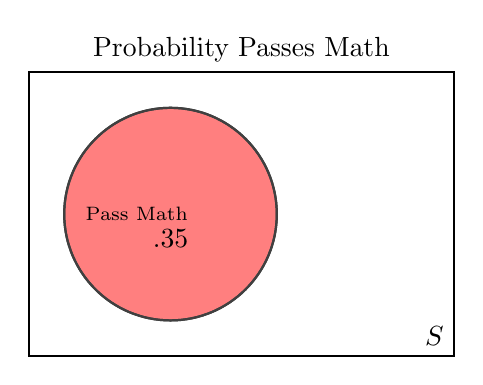
\begin{tikzpicture}[scale=.9]
	\def\circleA{(0,0) circle (1.5)} %A
	\def\circleB{(0:2) circle (1.5)} %B

	\colorlet{circle edgeA}{black!75} 
	\colorlet{circle areaA}{red!100}
	\colorlet{circle edgeB}{black!75} 
	\colorlet{circle areaB}{green!100}

	\tikzset{
		filledA/.style={fill=circle areaA, draw=circle edgeA, thick},
		filledB/.style={fill=circle areaB, draw=circle edgeB, thick},
		outlineA/.style={draw=circle edgeA, thick},
		outlineB/.style={draw=circle edgeB, thick},
	}
	
	\begin{scope}[fill opacity=0.5]         
			\fill[filledA] \circleA;
			%\fill[filledB] \circleB;    
	\end{scope}

	\draw[outlineA] \circleA node[left=-10pt] {\scriptsize Pass Math} node[below=2pt] {.35}; 
	%\draw[outlineB] \circleB node[right=-10pt] {\scriptsize Pass Art}; 
	\draw[thick] (-2,-2) rectangle (4,2) node[anchor=south east] at (current bounding box.south east) {$S$}; 
	\node[anchor=south] at (current bounding box.north) {Probability Passes Math}; 
\end{tikzpicture} }

 \only<4-8>{%%%% M or A %%%%%
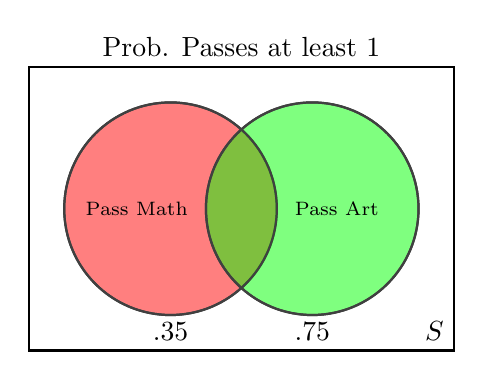
\begin{tikzpicture}[scale=.9]
	\def\circleA{(0,0) circle (1.5)} %A
	\def\circleB{(0:2) circle (1.5)} %B

	\colorlet{circle edgeA}{black!75} 
	\colorlet{circle areaA}{red!100}
	\colorlet{circle edgeB}{black!75} 
	\colorlet{circle areaB}{green!100}

	\tikzset{
		filledA/.style={fill=circle areaA, draw=circle edgeA, thick},
		filledB/.style={fill=circle areaB, draw=circle edgeB, thick},
		outlineA/.style={draw=circle edgeA, thick},
		outlineB/.style={draw=circle edgeB, thick},
	}
	
	\begin{scope}[fill opacity=0.5]         
			\fill[filledA] \circleA;
			\fill[filledB] \circleB;    
	\end{scope}

	\draw[outlineA] \circleA node[left=-10pt] {\scriptsize Pass Math} node[below=-1pt] at (0,-1.5) {.35}; 
	\draw[outlineB] \circleB node[right=-10pt] {\scriptsize Pass Art} node[below=-1pt] at (2,-1.5) {.75};
	%\draw (1,0) node {.25};
	\draw[thick] (-2,-2) rectangle (4,2) node[anchor=south east] at (current bounding box.south east) {$S$}; 
	\node[anchor=south] at (current bounding box.north) {Prob. Passes at least 1}; 
\end{tikzpicture} } \only<9-9>{%%%% M and A %%%%%
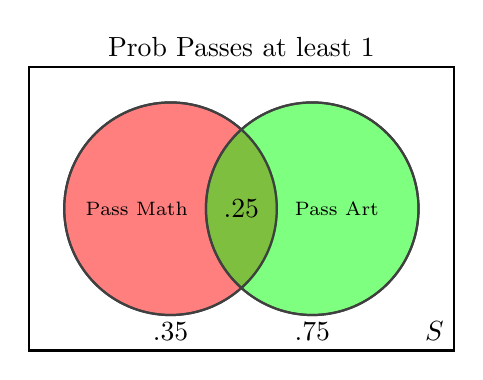
\begin{tikzpicture}[scale=.9]
	\def\circleA{(0,0) circle (1.5)} %A
	\def\circleB{(0:2) circle (1.5)} %B

	\colorlet{circle edgeA}{black!75} 
	\colorlet{circle areaA}{red!100}
	\colorlet{circle edgeB}{black!75} 
	\colorlet{circle areaB}{green!100}

	\tikzset{
		filledA/.style={fill=circle areaA, draw=circle edgeA, thick},
		filledB/.style={fill=circle areaB, draw=circle edgeB, thick},
		outlineA/.style={draw=circle edgeA, thick},
		outlineB/.style={draw=circle edgeB, thick},
	}
	
	\begin{scope}[fill opacity=0.5]         
			\fill[filledA] \circleA;
			\fill[filledB] \circleB;    
	\end{scope}

	\draw[outlineA] \circleA node[left=-10pt] {\scriptsize Pass Math} node[below=-1pt] at (0,-1.5) {.35}; 
	\draw[outlineB] \circleB node[right=-10pt] {\scriptsize Pass Art} node[below=-1pt] at (2,-1.5) {.75};
	\draw (1,0) node {.25};
	\draw[thick] (-2,-2) rectangle (4,2) node[anchor=south east] at (current bounding box.south east) {$S$}; 
	\node[anchor=south] at (current bounding box.north) {Prob Passes at least 1}; 
\end{tikzpicture} }\only<10-10>{%%%%MnA%%%%%
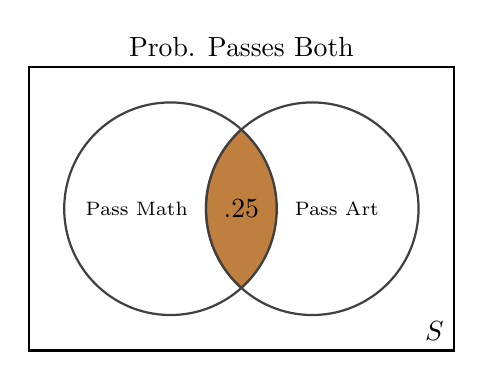
\begin{tikzpicture}[scale=.9]
	\def\circleA{(0,0) circle (1.5)} %A
	\def\circleB{(0:2) circle (1.5)} %B

	\colorlet{circle edgeA}{black!75} 
	\colorlet{circle areaA}{red!100}
	\colorlet{circle edgeB}{black!75} 
	\colorlet{circle areaB}{green!100}

	\tikzset{
		filledA/.style={fill=circle areaA, draw=circle edgeA, thick},
		filledB/.style={fill=circle areaB, draw=circle edgeB, thick},
		outlineA/.style={draw=circle edgeA, thick},
		outlineB/.style={draw=circle edgeB, thick},
	}
	
	\begin{scope}[fill opacity=0.5]    
		\clip \circleA;     
			\fill[filledB] \circleB;
		\clip \circleB;     
			\fill[filledA] \circleA;
	\end{scope}

	\draw[outlineA] \circleA node[left=-10pt] {\scriptsize Pass Math} node[below=-1pt] at (0,-1.5) {}; 
	\draw[outlineB] \circleB node[right=-10pt] {\scriptsize Pass Art} node[below=-1pt] at (2,-1.5) {};
	\draw (1,0) node {.25};

	%\node[anchor=south] at (current bounding box.north) {$A \cap B$}; 
	\draw[thick] (-2,-2) rectangle (4,2) node[anchor=south east] at (current bounding box.south east) {$S$};
	\node[anchor=south] at (current bounding box.north) {Prob. Passes Both};
\end{tikzpicture} }\only<11-14>{%%%%(MUA)' complement%%%%%
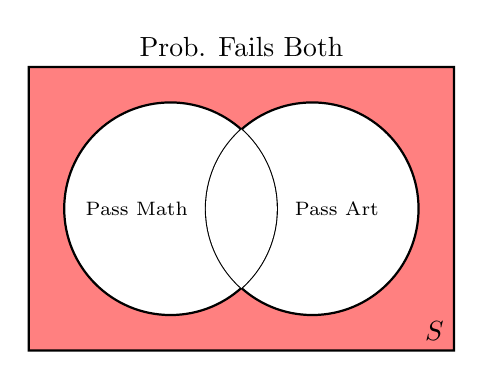
\begin{tikzpicture}[scale=.9]
	\def\circleA{(0,0) circle (1.5)} %A
	\def\circleB{(0:2) circle (1.5)} %B

	\colorlet{circle edgeA}{black!75} 
	\colorlet{circle areaA}{red!100}
	\colorlet{circle edgeB}{black!75} 
	\colorlet{circle areaB}{blue!100}

	\tikzset{
		filledA/.style={fill=circle areaA, draw=circle edgeA, thick},
		filledB/.style={fill=circle areaB, draw=circle edgeB, thick},
		outlineA/.style={draw=circle edgeA, thick},
		outlineB/.style={draw=circle edgeB, thick},
	}

		\draw[thick,fill=red!50,even odd rule] %%even odd rule draws complement of next draw commands%%
			(-2,-2) rectangle (4,2) node[anchor=south east] at (current bounding box.south east) {$S$}
			\circleA node[left=-10pt] {\scriptsize Pass Math} node[below=-1pt] at (0,-1.5) {}
			\circleB node[right=-10pt] {\scriptsize Pass Art} node[below=-1pt] at (2,-1.5) {};

		\scope 
			\clip (0,0) circle (1.5);%%why can't i use circleA?
			\fill[white] (0:2) circle (1.5); 
		\endscope
		
	\node[anchor=south] at (current bounding box.north) {Prob. Fails Both}; 

\end{tikzpicture} } \only<17-18>{%%%% M %%%%%
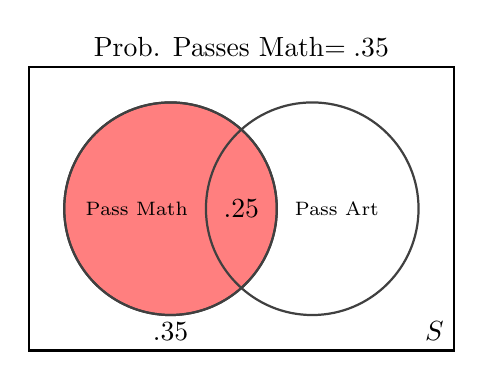
\begin{tikzpicture}[scale=.9]
	\def\circleA{(0,0) circle (1.5)} %A
	\def\circleB{(0:2) circle (1.5)} %B

	\colorlet{circle edgeA}{black!75} 
	\colorlet{circle areaA}{red!100}
	\colorlet{circle edgeB}{black!75} 
	\colorlet{circle areaB}{green!100}

	\tikzset{
		filledA/.style={fill=circle areaA, draw=circle edgeA, thick},
		filledB/.style={fill=circle areaB, draw=circle edgeB, thick},
		outlineA/.style={draw=circle edgeA, thick},
		outlineB/.style={draw=circle edgeB, thick},
	}
	
	\begin{scope}[fill opacity=0.5]         
			\fill[filledA] \circleA;
			%\fill[filledB] \circleB;    
	\end{scope}

	\draw[outlineA] \circleA node[left=-10pt] {\scriptsize Pass Math} node[below=-1pt] at (0,-1.5) {.35}; 
	\draw[outlineB] \circleB node[right=-10pt] {\scriptsize Pass Art} node[below=-1pt] at (2,-1.5) {};
	%\node[anchor=south] at (current bounding box.north) {$A \cup B$};
	\draw (1,0) node {.25};
	\draw[thick] (-2,-2) rectangle (4,2) node[anchor=south east] at (current bounding box.south east) {$S$};
	\node[anchor=south] at (current bounding box.north) {Prob. Passes Math$=.35$};
\end{tikzpicture} }\only<19-19>{%%%%M-A%%%%%
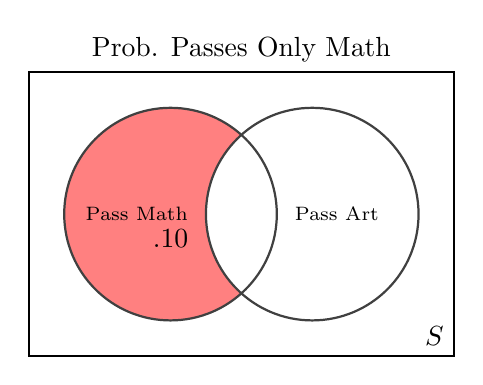
\begin{tikzpicture}[scale=.9]
	\def\circleA{(0,0) circle (1.5)} %A
	\def\circleB{(0:2) circle (1.5)} %B

	\colorlet{circle edgeA}{black!75} 
	\colorlet{circle areaA}{red!50}
	\colorlet{circle edgeB}{black!75} 
	\colorlet{circle areaB}{red!50}

	\tikzset{
		filledA/.style={fill=circle areaA, draw=circle edgeA, thick},
		filledB/.style={fill=circle areaB, draw=circle edgeB, thick},
		outlineA/.style={draw=circle edgeA, thick},
		outlineB/.style={draw=circle edgeB, thick},
	}
	
	\begin{scope}[fill opacity=1.0]    
		\fill[circle areaA] \circleA;
		\clip \circleA;     
			\fill[white] \circleB;
		%\clip \circleB;     
			%\fill[filledA] \circleA;
	\end{scope}

	\draw[outlineA] \circleA node[left=-10pt] {\scriptsize Pass Math} node[below=2pt] {.10}; 
	\draw[outlineB] \circleB node[right=-10pt] {\scriptsize Pass Art} node[below=-1pt] at (2,-1.5) {}; 
	\draw[thick] (-2,-2) rectangle (4,2) node[anchor=south east] at (current bounding box.south east) {$S$}; 
	\node[anchor=south] at (current bounding box.north) {Prob. Passes Only Math}; 
\end{tikzpicture} }\only<20-21>{%%%%A-M%%%%%
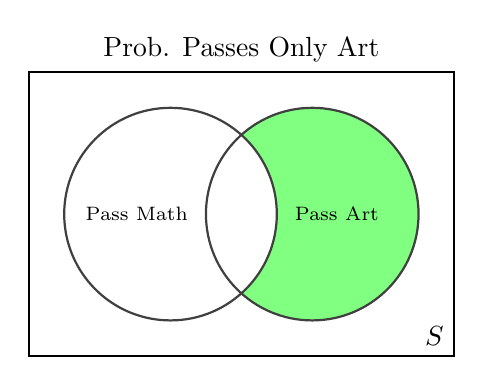
\begin{tikzpicture}[scale=.9]
	\def\circleA{(0,0) circle (1.5)} %A
	\def\circleB{(0:2) circle (1.5)} %B

	\colorlet{circle edgeA}{black!75} 
	\colorlet{circle areaA}{red!50}
	\colorlet{circle edgeB}{black!75} 
	\colorlet{circle areaB}{green!50}

	\tikzset{
		filledA/.style={fill=circle areaA, draw=circle edgeA, thick},
		filledB/.style={fill=circle areaB, draw=circle edgeB, thick},
		outlineA/.style={draw=circle edgeA, thick},
		outlineB/.style={draw=circle edgeB, thick},
	}
	
	\begin{scope}[fill opacity=1.0]    
		\fill[circle areaB] \circleB;
		\clip \circleA;     
			\fill[white] \circleB;
		%\clip \circleB;     
			%\fill[filledA] \circleA;
	\end{scope}

	\draw[outlineA] \circleA node[left=-10pt] {\scriptsize Pass Math} node[below=-1pt] at (0,-1.5) {}; 
	\draw[outlineB] \circleB node[right=-10pt] {\scriptsize Pass Art} node[below=2pt] {}; 
	\draw[thick] (-2,-2) rectangle (4,2) node[anchor=south east] at (current bounding box.south east) {$S$}; 
	\node[anchor=south] at (current bounding box.north) {Prob. Passes Only Art}; 
\end{tikzpicture} }\only<22->{%%%%(AuM)-(AnM)%%%%%
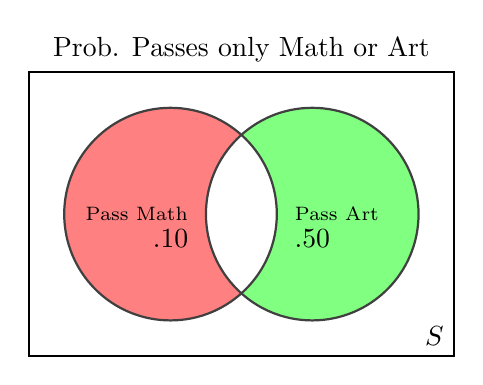
\begin{tikzpicture}[scale=.9]
	\def\circleA{(0,0) circle (1.5)} %A
	\def\circleB{(0:2) circle (1.5)} %B

	\colorlet{circle edgeA}{black!75} 
	\colorlet{circle areaA}{red!50}
	\colorlet{circle edgeB}{black!75} 
	\colorlet{circle areaB}{green!50}

	\tikzset{
		filledA/.style={fill=circle areaA, draw=circle edgeA, thick},
		filledB/.style={fill=circle areaB, draw=circle edgeB, thick},
		outlineA/.style={draw=circle edgeA, thick},
		outlineB/.style={draw=circle edgeB, thick},
	}
	
	\begin{scope}[fill opacity=1.0]    
		\fill[circle areaB] \circleB;
		\clip \circleA;     
			\fill[white] \circleB;
		%\clip \circleB;     
			%\fill[filledA] \circleA;
	\end{scope}

	\begin{scope}[fill opacity=1.0]    
		\fill[circle areaA] \circleA;
		%\clip \circleA;     
			%\fill[white] \circleB;
		\clip \circleB;     
			\fill[white] \circleA;
	\end{scope}

	\draw[outlineA] \circleA node[left=-10pt] {\scriptsize Pass Math} node[below=2pt] {.10}; 
	\draw[outlineB] \circleB node[right=-10pt] {\scriptsize Pass Art} node[below=2pt] {.50};  
	\draw[thick] (-2,-2) rectangle (4,2) node[anchor=south east] at (current bounding box.south east) {$S$}; 
	\node[anchor=south] at (current bounding box.north) {Prob. Passes only Math or Art}; 
\end{tikzpicture} }
\end{columns}
\vspace{.25cm}

\only<2-3>{Probability that a student does NOT fail Math: $1-.65$} \only<3-3>{$=.35$}

\only<5-10>{Probability that a student passes Math AND Art is: $P(M\cap A)$}

\only<6-10>{

\begin{tabular}{cccccccc}
\only<6->{ \textcolor{red}{Pass both$\downarrow$}} &  &  &  &  &  &  & \tabularnewline
$P(M\cup A)$ & $=$ & $P(M)$ & $+$ & $P(A)$ & $-$ & $P(M\cap A)$ & \tabularnewline
\only<6->{.85} & \only<6->{$=$} & \only<7->{$.35$} & \only<7->{$+$} & \only<8->{$.75$} & \only<8->{$-$} & \only<9->{$.25$} & \tabularnewline
\end{tabular}}\only<12-14>{Probability that a student does NOT pass at least
one.

\only<13-14>{ \hspace{1.5cm}$1-.85$} \only<14-14>{$=.15$}}

\only<16->{Probability that a student passes just Math} \only<20->{OR
just Art}

\only<17-19>{%
\begin{tabular}{ccccc}
$P(M)$ & $-$ & $P(M\cap A)$ &  & \tabularnewline
\only<18->{.35} & \only<18->{$-$} & \only<18->{.25} & \only<19->{$=.10$} & \tabularnewline
\end{tabular}}

\only<20-22>{%
\begin{tabular}{ccccc}
$P(A)$ & $-$ & $P(M\cap A)$ &  & \tabularnewline
\only<21->{.75} & \only<21->{$-$} & \only<21->{.25} & \only<21->{$=.5$} & \tabularnewline
\end{tabular}}

\only<23->{$.10+.50$} \only<24->{$=.60$}
\end{frame}

\end{document}
